% !TEX root = ../thesis.tex
%
\chapter{Hintergrund}
\label{sec:concepts}
In diesem Kapitel wird das Datenmodell von Wikidata beschrieben.
Danach wird das Format RDF\footnote{\url{https://www.w3.org/RDF/}} (Resource Description Framework) erläutert und die Abbildung von Wikidata auf dieses Format erklärt.
RDF ist Standardformat für den Austausch von strukturierten Informationen. 

\section{Wikidata als strukturiertes Wiki}
Wikidata ist die gemeinsame Wissensdatenbank der Wikimedia Projekte.
Wie Wikipedia selbst basiert Wikidata auf MediaWiki\footnote{\url{https://mediawiki.org}}, einer Software für das Betreiben von kollaborativen Wikis.
Statt Dokumenten in natürlicher Sprache verwaltet Wikidata jedoch strukturierte Dokumente.
Die Erweiterungen für MediaWiki stellt dazu das Wikibase\footnote{\url{htts://wikiba.se}} Projekt bereit.

Die Dokumentation von Wikibase \cite{wikibase-data-model} beschreibt das Datenmodell detailliert.
Alle Dokumente in Wikidata besitzen einen eindeutigen Identifier.
Dieser beginnt mit einem Großbuchstaben, der den Typ des Dokuments angibt, gefolgt von einer Zahl.
Aktuell kennt Wikidata drei Typen von Dokumenten: \introterm{Items} (Q), \introterm{Properties} (P) und \introterm{Lexemes} (L).
Lexemes wurden erst 2018 hinzugefügt, sind damit noch recht neu.
Da Wikidata-Toolkit diese noch nicht vollständig unterstützt, werden Lexemes im folgenden nicht genauer betrachtet.

Den Hauptbestandteil der Daten bilden die Items (Q).
Items repräsentieren Dinge, die durch Wikidata beschrieben werden.
In vielen Fällen existieren auch Wikipedia-Artikel in verschiedenen Sprachen zu dem Ding, welches durch das Item repräsentiert wird.
Zur Verlinkung zwischen Item und Seiten des Wikimedia Projekts (Wikipedia-Artikel, Wikiquote-Seiten etc.) enthält jedes Item eine Liste von \introterm{Sitelinks}.
Die Properties (P) stellen die Attribute dar, die zur Beschreibung von Items verwendet werden können.

Der Aufbau eines Items ist beispielhaft anhand von \verb|Q42| (Douglas Adams) in \cref{fig:wd-datamodel} dargestellt.
Den ersten Teil bilden die \introterm{Terme}: \introterm{Label}, \introterm{Description} und \introterm{Aliases}.
Diese dienen zur Beschreibung und Definition des Items.
Die Terme sind mehrsprachig: ein Item kann ein \introterm{Label} für viele verschiedene Sprachen haben.
Darauf folgen \introterm{Statements}, welche die Fakten zu diesem Item wiedergeben.
Den letzten Teil bilden die Sitelinks.
Die Sitelinks von \verb|Q42| verlinken zum Beispiel unter anderem auf Artikel von Douglas Adams in den unterschiedlichen Sprachversionen von Wikipedia und in Wikiquote.

Die Fakten eines Items werden in Statements beschrieben.
Ein Statement besteht aus zwei Teilen: einem \introterm{Claim}, der eine bestimmte Aussage trifft, und einer Liste von \introterm{Referenzen}.
Da Statements ohne Referenzen erlaubt sind, kann die Liste der Referenzen leer sein.
Jede Aussage enthält einen \introterm{Snak}.
Es gibt drei Arten von Snaks:
\begin{description}
\item[PropertyValue] die am meisten verwendete Art eines Snaks. Sie beschreibt den Fakt, dass eine bestimmte Eigenschaft (Property) einen gewissen Wert (Value) hat. Die Property bestimmt dabei den Typ der Value. Values können je nach Property andere Items oder skalare Werte (wie Zahlen, Zeichenketten, Koordinaten, Zeiten usw.) sein. Eine Liste der möglichen Typen zeigt \cref{tab:wd-datatypes}.
\item[SomeValue] diese Art Snak wird verwendet, um auszudrücken, dass ein Wert für die Eigenschaft existiert der aber nicht bekannt ist. Zum Beispiel kann der Snak "`es existiert ein Wert für den Todeszeitpunkt einer Person"' verwendet werden, falls eine Person gestorben ist, der Todeszeitpunkt aber nicht bekannt ist.
\item[NoValue] drückt aus, dass es für eine bestimmte Eigenschaft keinen Wert gibt. Diese Art Snak wird verwendet, wenn das Fehlen einer Information keine Unvollständigkeit darstellt. Kann zum Beispiel für \verb|P200| (Zuflüsse) verwendet werden, wenn ein Gewässer keine Zuflüsse besitzt. 
\end{description}
Der Claim eines Statements besteht aus einem \introterm{MainSnak} für die Hauptaussage und zusätzlichen \introterm{Qualifiern} zur Verfeinerung der Aussage.
Eine Referenz ist einfach eine Liste von Snaks. 

Ein MainSnak zu Douglas Adams (Q42) ist zum Beispiel \verb|P69| (educated at) - \verb|Q691283| (St John's College).
Mit den Qualifier-Snaks wie \verb|P582| (end time) - \verb|1974| bildet dieser dann einen Claim.
Das Statement setzt sich dann aus diesem Claim und der Liste von Referenzen zusammen.
Alle Statements für die gleiche Property werden in einer \introterm{Statement Group} zusammengefasst.
Jedes Statement besitzt einen \introterm{Rank} (\introterm{Deprecated}, \introterm{Normal} oder \introterm{Best}) um die Priorität innerhalb der Statement Group auszudrücken.

Dieses dokumentorientierte Datenmodell lässt sich einfach als JSON\footnote{\url{https://www.json.org}} (JavaScript Object Notation) repräsentieren.
Die vollständige Darstellung ist jedoch sehr umfangreich und ist deshalb aus Platzgründen hier nicht abgebildet.
Für ein Entity kann die JSON-Repräsentation einfach online abgerufen werden, für \verb|Q42| zum Beispiel unter: \url{https://www.wikidata.org/wiki/Special:EntityData/Q42.json}.

Wikidata erstellt wöchentlich einen \introterm{Gesamtexport} der Daten als JSON-Liste von Dokumenten.
Unter \url{https://dumps.wikimedia.org/wikidatawiki/entities/} lassen sich diese Exporte als GZip\footnote{\url{http://www.gzip.org/}} (58 GiB\footnote{die Zahlen wurden am 18.10.2019 ermittelt}) oder BZip2\footnote{\url{https://sourceforge.net/projects/bzip2/}} (39 GiB) komprimierte Dateien herunterladen.
Der GZip-Export ist zwar etwas größer, dafür ist der Aufwand zur Dekompression geringer, sodass die Geschwindigkeit der Verarbeitung schneller ist.

\begin{figure}
  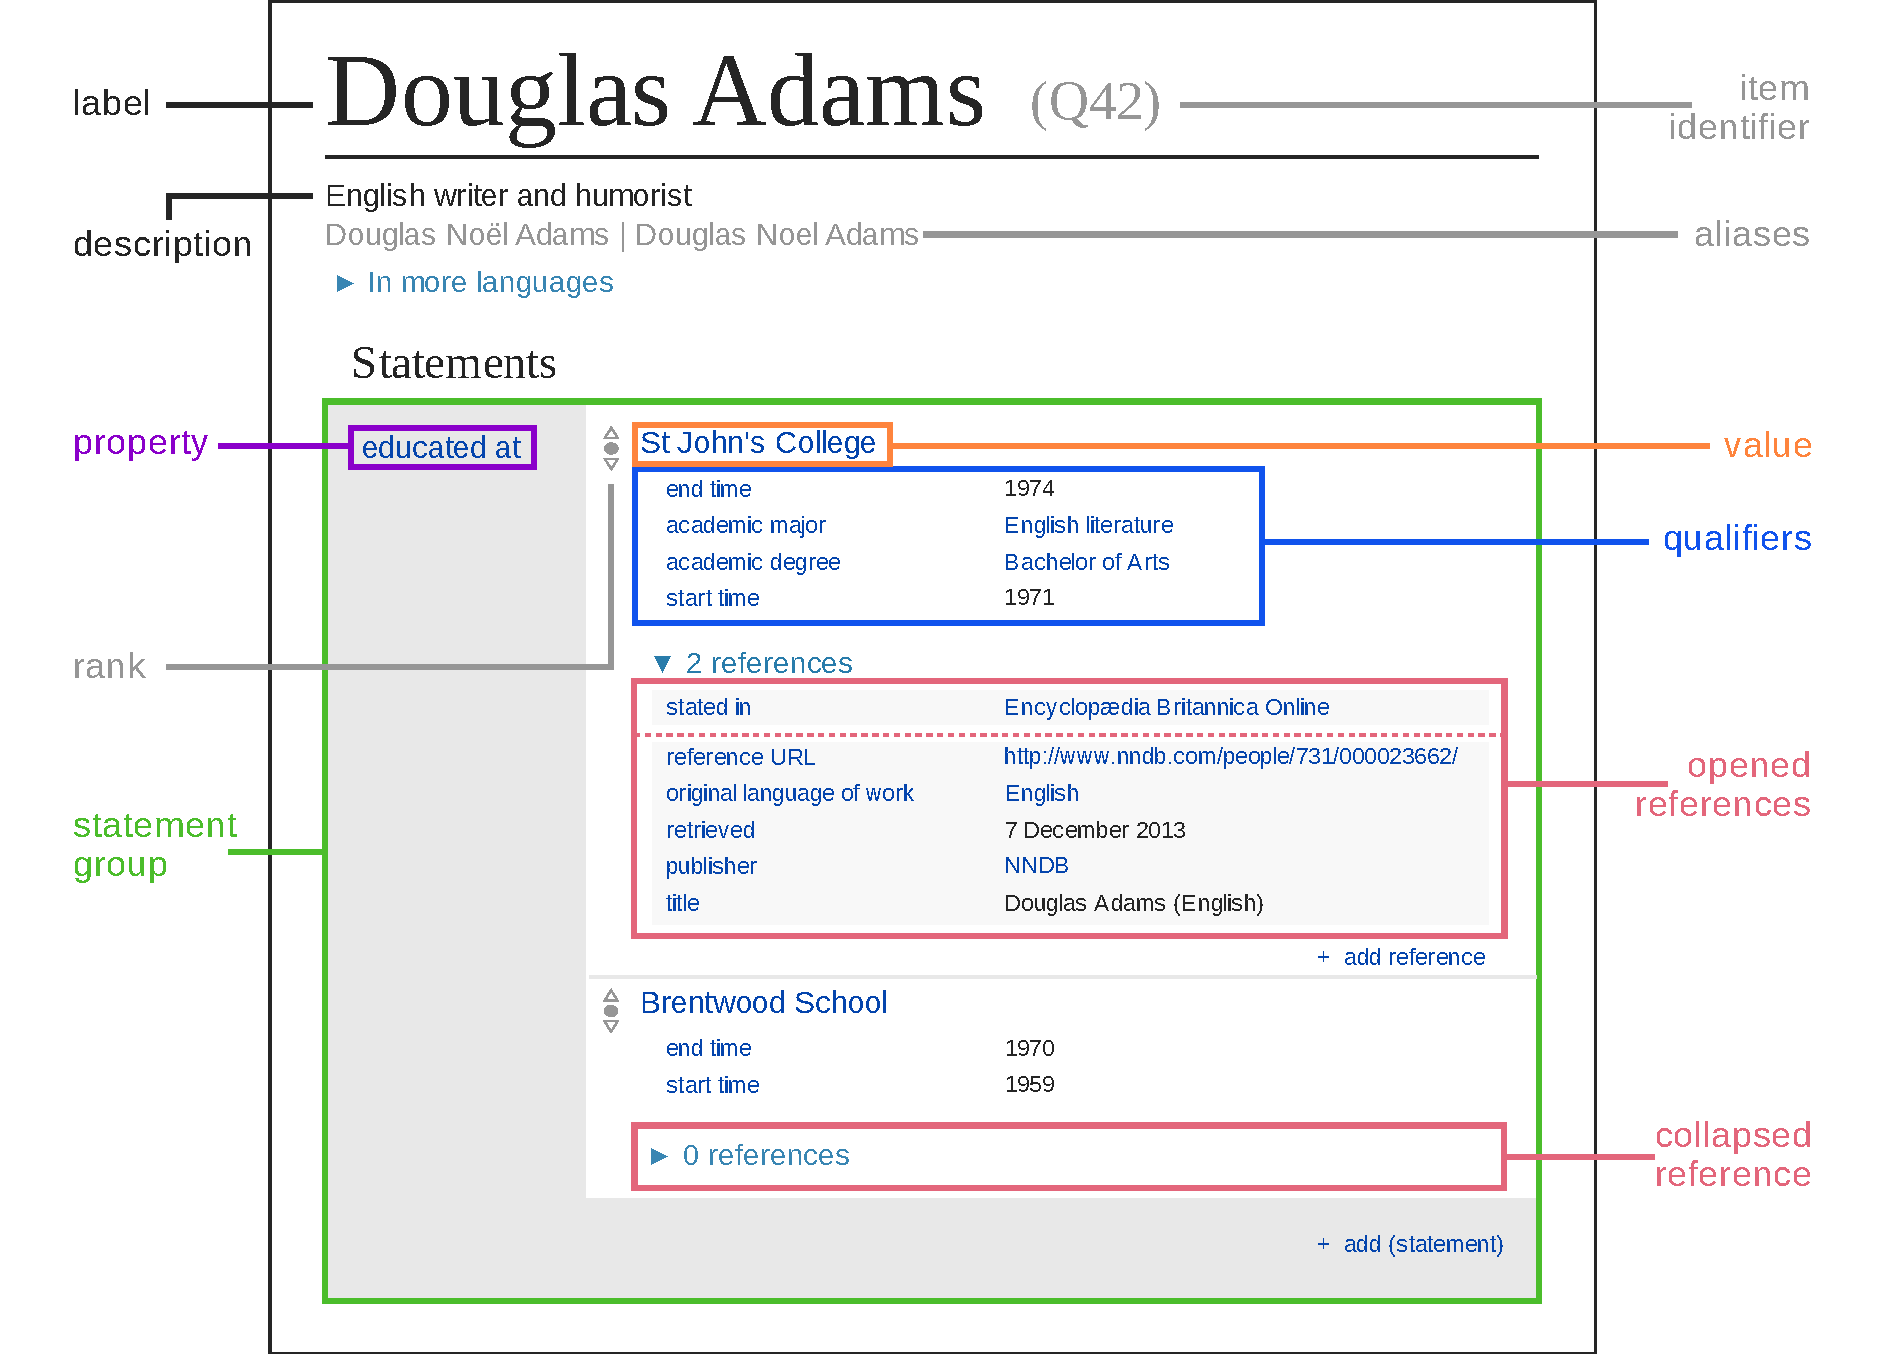
\includegraphics[width=\linewidth]{pics/Datamodel_in_Wikidata}
  \caption[Wikidata Item "`Q42"']{Wikidata Item "`Q42"'. \\ \small{Bild aus \url{https://www.mediawiki.org/wiki/Wikibase/DataModel/Primer\#/media/File:Datamodel_in_Wikidata.svg}}}
  \label{fig:wd-datamodel}
\end{figure}

\begin{table}
  \setlength{\extrarowheight}{0.1cm}
  \begin{adjustwidth}{-1cm}{-1cm}
    \begin{minipage}{\textwidth}
    \begin{tabular}{l p{0.75\textwidth} p{0.1\textwidth}}
      \bfseries{Typ}   & \bfseries{Beschreibung}                                                                                                                                       & \bfseries{Attribute} \\
      String           & Zeichenkette (ohne Sprachangabe)                                                                                                                              & nein \\
      Monolingualtext  & Zeichenkette (mit Angabe der Sprache)                                                                                                                         & nein \\
      WikibaseItem     & Ein Wikidata Item                                                                                                                                             & nein \\
      WikibaseProperty & Eine Wikidata Property                                                                                                                                        & nein \\
      ExternalId       & Ein Bezeichner in einer anderen Datenbank\newline{}
                         Mit P1630 (formatter URL) wird bei Properties von diesem Typ ein Format zur Erzeugung von URLs aus dem Bezeichner angegeben                                   & nein \\
      Url              & Eine URL zur Identifikation einer externen Resource. Beispiele sind Webseiten (\verb|http:|), Email-Adressen (\verb|mailto:|) oder IRC channel (\verb|irc:|)  & nein \\
      Math             & Eine mathematische Formel; das Format ist ein MediaWiki-spezifisches Subset von \LaTeX\footnote{\url{https://en.wikipedia.org/wiki/Help:Displaying_a_formula}}& nein \\
      MusicalNotation  & Eine Sequenz von Noten; Werte mit diesem Typ sind Zeichenketten in der LilyPond\footnote{\url{http://lilypond.org/}}-Notation                                 & nein \\
      CommonsMedia     & Referenz auf eine Mediendatei in Wikimedia Commons                                                                                                            & nein \\
      TabularData      & Referenz auf eine Tabelle in Wikimedia Commons                                                                                                                & nein \\
      GeoShape         & Referenz auf Kartendaten (\verb|.map|) in Wikimedia Commons                                                                                                   & nein \\
      Quantity         & Eine Zahlenangabe; neben der Zahl selbst (\verb|amount|) kann optional eine untere (\verb|upperBound|) und untere (\verb|lowerBound|) Schranke für das
                         Interval der Unsicherheit angegeben werden; außerdem wird eine Einheit \verb|unit| gespeichert (diese kann für dimensionslose Werte leer sein)                & \verb|amount|\newline{}
                                                                                                                                                                                         \verb|upperBound|\newline{}
                                                                                                                                                                                         \verb|lowerBound|\newline{}
                                                                                                                                                                                         \verb|unit| \\
      Time             & Ein Zeitpunkt; \verb|time| ist ein Zeitstempel in einem an ISO 8601 angelehnten Format (Beispiel: +2013-01-01T00:00:00Z);
                         \verb|precision| gibt Präzision der Angabe an (100 Millionen Jahre (1), \ldots, Jahrhundert (7), Dekade (8), Jahr (9), Monat (10), Tag (11), \ldots);
                         \verb|before| und \verb|after| geben die Ungenaugkeit der Angabe an (Einheit abhängig von \verb|precision|);
                         \verb|timezone| spezifiziert die Zeitzone, \verb|calendarmodel| das Kalendermodell (momentan werden gregorianisch und julianische Kalender untersüztzt)            & \verb|time|\newline{}
                                                                                                                                                                                         \verb|before|\newline{}
                                                                                                                                                                                         \verb|after|\newline{}
                                                                                                                                                                                         \verb|precision|\newline{}
                                                                                                                                                                                         \verb|timezone|\newline{}
                                                                                                                                                                                         \verb|calendarmodel| \\
      GlobeCoordinate  & Geographische Position; \verb|latitute| und \verb|longtitude| geben die Koordinaten an; \verb|globe| spezifiziert den Planet (Standard: \verb|Q2| (Erde));
                         \verb|precision| speichert die numerische Präzision der Koordinatenangaben; als Koordinatensystem wird das World Geodetic System (WGS84) angenommen           & \verb|latitude|\newline{}
                                                                                                                                                                                         \verb|longtitude|\newline{}
                                                                                                                                                                                         \verb|globe|\newline{}
                                                                                                                                                                                         \verb|precision| \\
      WikibaseLexeme   & Ein Wikidata Lexeme                                                                                                                                           & nein \\
      WikibaseSense    & Ein Wikidata Sense (Teil von Lexemes)                                                                                                                         & nein \\
      WikibaseForm     & Wikidata Form (Teil von Lexemes)                                                                                                                              & nein
    \end{tabular}
    \end{minipage}
  \end{adjustwidth}
  \caption{Datentypen in Wikidata. Eine Beschreibung dieser Datentypen ist unter \url{https://www.wikidata.org/w/index.php?title=Help:Data_type&oldid=1027592722} abrufbar}
  \label{tab:wd-datatypes}
\end{table}

\section{Resource Description Framework}
Eine Besonderheit von Wikidata ist die starke Verlinkung der Daten untereinander.
Diese Verlinkung ermöglicht eine Art des Zugriffs, die sich von der dokumentbasierten Betrachtungsweise unterscheidet.
Fragestellungen wie "`Wer sind die Verwandten von Douglas Adams?"' oder "`Welche berühmten Personen sind in einem Staat geboren, der Mitglied der Europäischen Union ist?"' betrachten die Beziehungen der Dokumente und nicht allein den Inhalt einzelner Dokumente.

Das W3C hat für solche Graph-basierten Daten RDF entwickelt \cite{rdf-spec}.
In RDF werden als eindeutige Bezeichner Internationalized Resource Identifiers (IRIs)\footnote{https://www.ietf.org/rfc/rfc3987.txt} verwendet.
IRIs sind eine Erweiterung von URIs zur Unterstützung von internationalen Zeichensätzen.
In der Praxis werden für IRIs oft HTTP URLs verwendet, sodass Namenskonflikte zwischen unterschiedlichen Organisationen vermieden werden.
Außerdem können über HTTP weitere Informationen zu der entsprechenden Ressource bereitgestellt werden.

Das Kernelement von RDF bilden Tripel. Die drei Komponenten jedes Tripel sind:
\begin{description}
\item[Subjekt] eine IRI oder Blank Node
\item[Prädikat] eine IRI
\item[Objekt] eine IRI, Blank Node oder Literal
\end{description}
Blank Nodes sind lokale Bezeichner, die im Gegensatz zu IRIs nur innerhalb eines Dokuments eindeutig sein müssen.
Verschiedene RDF Dokumente können daher die selben Blank Node Bezeichner verwenden, ohne dass damit die selbe Ressource beschrieben wird.

Literale in RDF bestehen aus einer Zeichenkette und optional noch einem Datentypen oder einem Language Tag.
Mit dem Datentyp kann die Interpretation der Zeichenkette genauer spezifiziert werden.
Datentypen werden über IRIs identifiziert.
Language Tags geben die Sprache der Zeichenkette als Language Code nach BCP47\footnote{\url{https://tools.ietf.org/html/bcp47}} an.
In diesem Fall muss der Datentyp \url{http://www.w3.org/1999/02/22-rdf-syntax-ns#langString} sein \cite{rdf-spec} .

RDF Dokumente sind eine ungeordnete Kollektion von Tripeln.
Für die Serialisierung von RDF gibt es verschiedene Standards, ein einfacher und verbreiteter ist N-Triples \cite{rdf-ntriples}.
Die Syntax von N-Triples ist in folgendem Beispiel dargestellt:
\begin{lstlisting}[language=SPARQL, breaklines=true]
<https://example.org> <http://schema.org/name> "Beispiel"@de .
<https://example.org> <http://schema.org/name> "Example"@en .
_:paper <https://example.org/about> <https://example.org> .
_:paper <https://example.org/popularity> "42"^^<http://www.w3.org/2001/XMLSchema#integer> .
\end{lstlisting}
Jede Zeile entspricht einem Tripel und wird mit einem Punkt abgeschlossen.
In N-Triples werden IRIs in \verb|<>| eingeschlossen und Blank Nodes durch das Präfix \verb|_:| markiert.
Literale sind von doppelten Anführungszeichen umgeben, mit einem At-Zeichen (\verb|@|) bzw. doppeltem Zirkumflex (\verb|^^|) können Language Tag und Datentyp angegeben werden.

In dieser Arbeit wird zur Übersichtlichkeit eine Erweiterung der Notation verwendet.
Dabei werden IRIs durch die Einführung von den in \cref{tab:rdf-prefixes} aufgeführten Präfixen vereinfacht.
Zum Beispiel wird \verb|<http://schema.org/name>| als \verb|schema:name| abgekürzt. 

\begin{table}
\begin{tabular}{l l}
\bfseries{Präfix} & \bfseries{URL} \\
rdf: & <http://www.w3.org/1999/02/22-rdf-syntax-ns\#> \\
xsd: & <http://www.w3.org/2001/XMLSchema\#> \\
% ontolex: & <http://www.w3.org/ns/lemon/ontolex\#> \\
% dct: & <http://purl.org/dc/terms/> \\
rdfs: & <http://www.w3.org/2000/01/rdf-schema\#> \\
owl: & <http://www.w3.org/2002/07/owl\#> \\
skos: & <http://www.w3.org/2004/02/skos/core\#> \\
schema: & <http://schema.org/> \\
% cc: & <http://creativecommons.org/ns\#> \\
geo: & <http://www.opengis.net/ont/geosparql\#> \\
prov: & <http://www.w3.org/ns/prov\#> \\
wikibase: & <http://wikiba.se/ontology\#> \\
wdata: & <http://www.wikidata.org/wiki/Special:EntityData/> \\
% bd: & <http://www.bigdata.com/rdf\#> \\
wd: & <http://www.wikidata.org/entity/> \\
wdt: & <http://www.wikidata.org/prop/direct/> \\
wdtn: & <http://www.wikidata.org/prop/direct-normalized/> \\
wds: & <http://www.wikidata.org/entity/statement/> \\
p: & <http://www.wikidata.org/prop/> \\
wdref: & <http://www.wikidata.org/reference/> \\
wdv: & <http://www.wikidata.org/value/> \\
ps: & <http://www.wikidata.org/prop/statement/> \\
psv: & <http://www.wikidata.org/prop/statement/value/> \\
psn: & <http://www.wikidata.org/prop/statement/value-normalized/> \\
pq: & <http://www.wikidata.org/prop/qualifier/> \\
pqv: & <http://www.wikidata.org/prop/qualifier/value/> \\
pqn: & <http://www.wikidata.org/prop/qualifier/value-normalized/> \\
pr: & <http://www.wikidata.org/prop/reference/> \\
prv: & <http://www.wikidata.org/prop/reference/value/> \\
prn: & <http://www.wikidata.org/prop/reference/value-normalized/> \\
wdno: & <http://www.wikidata.org/prop/novalue/>
\end{tabular}
\caption{Verwendete Präfixe. Alle Präfixe werden auch vom Wikidata Query Service vordefiniert.}
\label{tab:rdf-prefixes}
\end{table}

\section{Wikidata als RDF}
Als Standardformat für Graphdaten ist RDF weit verbreitet.
Um existierende Anwendungen mit den Daten von Wikidata verwenden zu können, ist eine Darstellung als RDF sinnvoll.
Eine direkte Abbildung von Statements auf Tripel ist jedoch nicht möglich, da RDF das Konzept von Qualifiern und Referenzen nicht kennt.
Außerdem erlaubt Wikidata mehrere Statements mit identischem Inhalt, was in RDF nicht vorgesehen ist.

Erxleben, Günther, Krötzsch, Mendez und Vrandečić haben 2014 beschrieben wie trotzdem eine Darstellung als RDF möglich ist und ein System zur Erstellung regelmäßiger Exporte als RDF entwickelt \cite{wikidata-rdf-export}.
Nach dem Prinzip der Reifikation werden Statements, Referenzen und komplexe Werte nicht direkt als Tripel exportiert, sondern als eigene Ressourcen. 
Diese Ressourcen besitzen dann ein Tripel, das zu dem Objekt des Statements verlinkt und zusätzlich noch Tripel für Qualifier und Referenzen.
Jedes Statement hat somit einen eindeutigen Namen, sodass auch zwei Statements mit dem selben Inhalt erfasst werden können.
\begin{figure}
  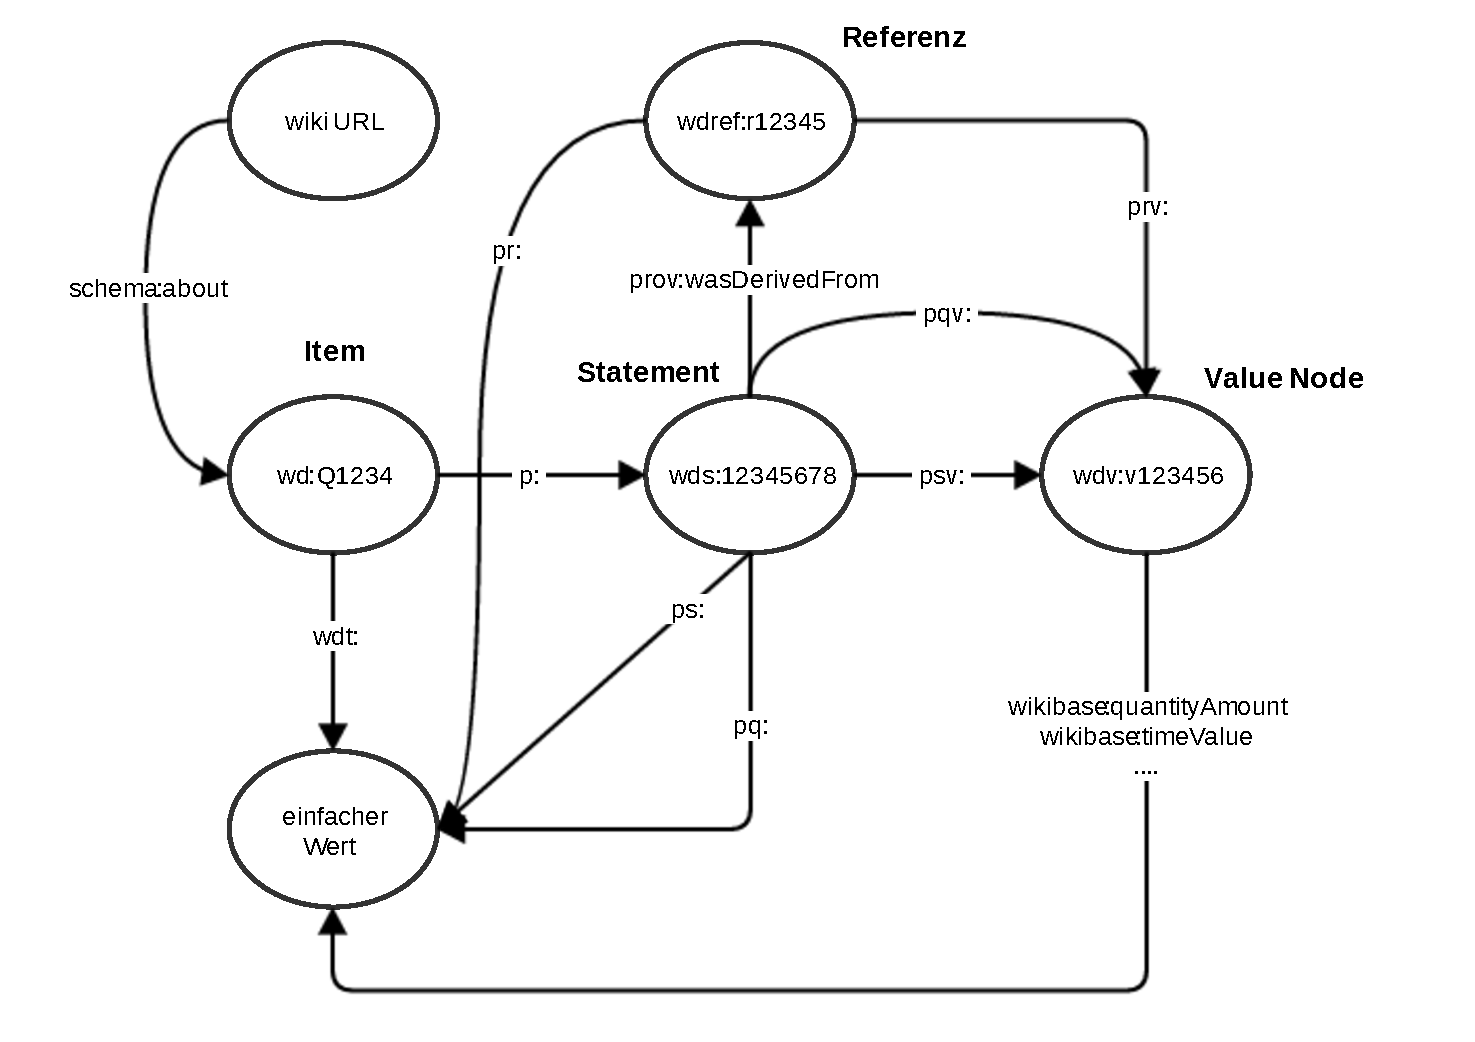
\includegraphics[width=\linewidth]{pics/Rdf_mapping}
  \caption{Mapping des Datenmodells auf RDF \\ Quelle für das Bild: \url{https://www.mediawiki.org/wiki/Wikibase/Indexing/RDF_Dump_Format\#/media/File:Rdf_mapping-vector.svg}}
  \label{fig:rdf-mapping}
\end{figure}

Diese Übersetzung ist in \cref{fig:rdf-mapping} gezeigt.
Jeder Pfeil beschreibt dabei Prädikatpräfix, welches für RDF-Tripel verwendet wird.
An dieses Präfix wird der Bezeichner der Property angehangen.
Hier ist ein Beispiel zur Verdeutlichung (gekürzt, die Informationen zu den Reference und Value Nodes sind nicht abgebildet):
\begin{lstlisting}[language=SPARQL]
wd:Q42 p:P26 wds:q42-xxxx .
wds:q42-xxxx rdf:type wikibase:Statement .
wds:q42-xxxx ps:P26 wd:Q14623681 .
wds:q42-xxxx pq:P580 "1991-11-25T00:00:00Z"^^xds:dateTime .
wds:q42-xxxx pqv:P580 wdv:c8ae0d38443d4671d3f893d7000a859e .
wds:q42-xxxx pq:P582 "2001-05-11T00:00:00Z"^^xsd:dateTime .
wds:q42-xxxx pqv:P582 wdv:1c30ade7914d072877b2db404a683d7c .
wds:q42-xxxx prov:wasDerivedFrom wdref:yyyyyyyy .
wd:Q42 wdt:P26 wd:Q14623681 .
\end{lstlisting}
Das Beispiel zeigt, wie die Property \verb|P26| (spouse) zuerst mit dem Prädikat \verb|p:P26| auf das Statement verlinkt.
Das Statement verlinkt über \verb|ps:P26| zum einfachen Wert der Property.
Mit \verb|pq:P580| (start time) bzw. \verb|pqv:P580| wird auf die einfache und komplexe Darstellung des Wertes für diesen Qualifier verlinkt.
Die komplexe Darstellung enthält noch weitere Informationen zu dem Datum, wie bspw. die Genauigkeit oder das verwendete Kalendermodell.

Eine spezielle Bedeutung hat der \verb|wdt:| Präfix.
Tripel mit diesen Prädikaten verlinken Items direkt mit den einfachen Werten.
Diese Tripel existieren allerdings nur dann, wenn das zugehörige Statement vom Typ \verb|BestRank| ist.
Dieser Typ umfasst alle Statements, die den höchsten Rang für diese Property haben und nicht deprecrated sind.
Solche Statements und Tripel werden auch als "`truthy"' bezeichnet.
In vielen Fällen können Abfragen damit deutlich kürzer und zugleich lesbarer formuliert werden, da einfache Verbindungen oft unabhängig von Qualifiern oder Referenzen betrachtet werden.

Auf Basis dieses Schemas hat Wikidata ein offizielles Format für Exporte als RDF entwickelt \footnote{\url{https://www.mediawiki.org/wiki/Wikibase/Indexing/RDF_Dump_Format}}.
Analog zu den Exporten im JSON-Format werden wöchentlich Gesamtexporte aller Daten als RDF erzeugt und zum Download angeboten.
Da RDF die Informationen weniger kompakt repräsentiert als JSON, sind die Exporte etwas größer: 76 GiB mit BZip2 und 99 GiB mit GZip.
Zusätzlich zu den vollständigen Exporten wird auch ein Export mit nur den truthy Tripeln angeboten, welcher deutlich kleiner ausfällt (32 GiB mit GZip).

Ein prominenter Nutzer des RDF-Formats ist der Wikidata Query Service\footnote{\url{https://query.wikidata.org}} \cite{wd-sparql}.
Auf Basis der RDF-Datenbank BlazeGraph\footnote{\url{https://blazegraph.com/}} wird ein Interface zum Abfragen der Daten mittels SPARQL bereitgestellt.
Die Daten werden initial aus dem RDF-Gesamtexport geladen und dann laufend mit der Wikidata-API inkrementell aktualisiert, sodass immer der aktuelle Stand abrufbar ist.